\subsection{FOV grid distortion}
\label{se:grid_distortion}

{\bf LP edit using Samuel's comments, [TBC]}

We studied the matching of the KIDs position on the sky to the
\emph{design} position, as decribed in Xavier's wiki post\footnote{see
  {\tt http$://$www.iram.fr$/$wiki$/$nika2$/$index.php$/$}
  
  {\tt April$\_$19,$\_$2017,$\_$FXD,$\_$KID$\_$position$\_$mapping$\_$and$\_$Field$\_$distortion$\_$for$\_$Run9}
}

This has been compared to expectations obtained using ZEMAX
simulation. The grid diagram generated using ZEMAX provides us with
the maximum dispersion in the field defined by

\begin{equation}
P = \frac{\sqrt{(x_p - x_r)^2 + (y_p - y_r)^2}}{\sqrt{x_p^2 + y_p^2}},
\end{equation}

where $(x_p, y_p)$ and $(x_r, y_r)$ are respectivelly the predicted
and real coordinates on the image surface relative to the reference
field position image location (see page 170 of the ZEMAX manual, 2007).
The predicted coordinates for the whole field are obtained using a
linear interpolation of a small area in the field central part,
whereas the real coordinates are calculated by ray tracing through the
optical system.

\begin{figure}[ht] 
\begin{center}
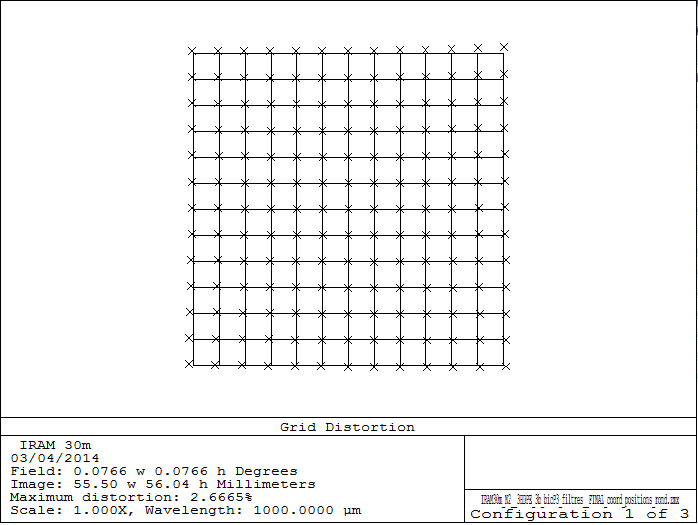
\includegraphics[width=0.9\textwidth]{Figures/NIKA2_Final_grid.png}
\caption{NIKA2 grid diagram simulated using ZEMAX. Crosses indicate
  the real coordinates on the Nasmyth image plan. {\bf question a
    Samuel: pourquoi les dimensions indiquees sont environs 4.5 arcmin
  de cote (et pas 6.5)?}}
 \label{fig:fov_grid_distortion_zemax}
\end{center}
\end{figure}

Figure \ref{fig:fov_grid_distortion_zemax} show the ZEMAX grid diagram for
NIKA2 simulated optic system. The maximum grid distortion is expected
to be of $2.7\%$ in NIKA2 $6.5'$ FOV. The distortion is the most
noticeable in the upper right corner of the Nasmyth plan, which is
also the area of the largest defocus w.r.t. to the center. 

